\documentclass[12pt, a4paper]{article}

\usepackage[hmargin=2.5cm, vmargin=2cm]{geometry}
\usepackage{amsthm, amssymb, mathtools, yhmath, graphicx}
\usepackage{fontspec, type1cm, titlesec, titling, fancyhdr, tabularx}
\usepackage{color, unicode-math, float, hhline}
\usepackage{parskip}

\usepackage[abbreviations, per-mode=symbol]{siunitx}
\usepackage[CheckSingle, CJKmath]{xeCJK}
\usepackage{CJKulem}
\usepackage{enumitem}
\usepackage{tikz}
\usepackage{circuitikz}
\usepackage{fancyvrb, hyperref}
\usepackage{etoolbox}
\AtBeginEnvironment{Verbatim}{\vspace{-12pt}}
\AtEndEnvironment{Verbatim}{\vspace{2pt}}
%\setCJKmainfont[BoldFont=cwTex Q Hei]{cwTex Q Ming}
%\setCJKsansfont[BoldFont=cwTex Q Hei]{cwTex Q Ming}
%\setCJKmonofont[BoldFont=cwTex Q Hei]{cwTex Q Ming}
\setCJKmainfont[BoldFont=cwTeX Q Hei]{cwTeX Q Ming}

\def\normalsize{\fontsize{12}{18}\selectfont}
\def\large{\fontsize{14}{21}\selectfont}
\def\Large{\fontsize{16}{24}\selectfont}
\def\LARGE{\fontsize{18}{27}\selectfont}
\def\huge{\fontsize{20}{30}\selectfont}

%\titleformat{\section}{\bf\Large}{\arabic{section}}{24pt}{}
%\titleformat{\subsection}{\large}{\arabic{subsection}.}{12pt}{}
%\titlespacing*{\subsection}{0pt}{0pt}{1.5ex}

\parindent=0pt
\parskip=16pt

\DeclarePairedDelimiter{\abs}{\lvert}{\rvert}
\DeclarePairedDelimiter{\norm}{\lVert}{\rVert}
\DeclarePairedDelimiter{\inpd}{\langle}{\rangle}
\DeclarePairedDelimiter{\ceil}{\lceil}{\rceil}
\DeclarePairedDelimiter{\floor}{\lfloor}{\rfloor}

\newcommand{\img}{\mathsf{i}}
\newcommand{\ex}{\mathsf{e}}
\newcommand{\dD}{\mathrm{d}}
\newcommand{\dI}{\,\mathrm{d}}

\title{平面顯示技術導論 HW \#2}
\author{B02901178 江誠敏}

\begin{document}


\maketitle

\begin{enumerate}[label={\arabic*.}, leftmargin=0pt]
  \item {An equivalent circuit of a single LCD pixel is shown below.
      The transistor will be replaced by a $\SI{50}\ohm$ resistor 
      which is connected between $V_s$ and $V_d$.  
      Assuming $C_{st}= \SI{3}{\pico\farad}$, and $C_{lc}=\SI{5}{\pico\farad}$,
      a step function $V_G$ is applied at $t=0$ to turn on the TFT, $V_D=0$ (at 
      $t<0$), $V_S=\SI{5}\V$. }

    \begin{enumerate}[label={(\alph*)}]
      \item Please calculate how long it takes to charge up $C_{lc}$ from $\SI{0}\V$ to $90\%$ of $V_s$
        (i.e. $\SI{4.5}\V$).

        {\bf Ans: } First we calculate the time constant $\tau = R (C_{lc} + C_{st}) = \SI{0.4}\ns$.
        \[ \ex^{-t/\tau} = 1 - 0.9 \quad \Rightarrow \quad t = \tau \log 10 \quad 
          \Rightarrow \quad t \approx \SI{0.92}\ns \]

      \item Please calculate how long it takes to charge up $C_{lc}$ from $\SI{0}\V$ 
        to $\SI{4.5}\V$ if $V_s$ becomes $\SI{9}\V$.

        {\bf Ans: } The time constant remains the same, but now $\SI{4.5}\V$ is only
        $50\%$ of $\SI{9}\V$.
        \[ \ex^{-t/\tau} = 1-0.5 \quad \Rightarrow \quad t = \tau \log 2 \quad 
          \Rightarrow \quad t \approx \SI{0.277}\ns \]

      \item Please comment on the overdrive technology.

        {\bf Ans: } The overdrive technology would give better respond speed, since
        its charging time is shorter.
    \end{enumerate}
  \item Questions:
    \begin{enumerate}[label={(\alph*)}]
      \item What is the duration (time), $T_3$, of the scan line 110?
        And what is $(t_2 - t_1)$ when the data line is enabled? \\
        {\bf Ans: }
        If $320 \times 120$ means that there are $320$ scan lines, then
        \[ T_3 = \SI{1}\s / 30 / 320  \quad \approx \SI{104.2}\us, \]
        Else
        \[ T_3 = \SI{1}\s / 30 / 120  \quad \approx \SI{277.8}\us. \]

        No matter what, we have
        \[ (t_2 - t_1) = \SI{1}\s / 30 / 120 / 320 \quad \approx \SI{0.868}\us \]

      \item What is the maximum capacitance of capacitor 104? \\
        {\bf Ans: } Let $\Delta t = (t_2 - t_1)/2, \tau = RC$ where $R = \SI{10}\ohm$.
        \begin{align*}
          & \ex^{-\Delta t/\tau} \leq 1 - 0.8 \; \implies \; \frac{\Delta t}{\tau} \geq \log 5 
          \; \implies \; RC = \tau \leq \frac{\Delta t}{\log 5} \\
          & \implies \; C \leq \frac{\Delta t}{R \log 5} 
          = \frac{t_2 - t_1}{2 R \log 5} \approx \SI{27.0}{\nano\farad} 
        \end{align*}

      \item Assuming the first OLED selected in the columns, after the data line 
        is disable, the circuit is in the discharge process.   Can the fully-on 
        period of the OLED last the entire scan line period ($T_3$)? \\
        {\bf Ans: } No, from the previous question we knew that
        \[ \tau \leq \frac{\Delta t}{\log 5} \]
        Let $V^*$ be the voltage of capacitor 104 just after the data line is disabled, and
        we know that $V^* \leq V_{\text{data}}$.
        Let $t^*$ be the time needed for the voltage to drop to $0.8 V_{\text{data}}$, which
        is greater than $0.8 V^*$, then
        \[ t^* \leq \tau (- \log 0.8) = \frac{\log 5/4}{\log 5} \Delta t \approx 0.14 \,\Delta t, \]
        Which is much smaller than $2 \Delta t = t_2 - t_1$, and not to mention $T_3$.
      \item Please plot (hand draw is OK) $I_{\text{OLED}}$ vs. time once 
        $V_{\text{data}}$ is enabled. \\
        We knew that $V_{104} = V_{\text{data}} (1 - \ex^{-t/\tau})$ from the previous problems.
        And we assume that $I_{\text{OLED}} \propto V_{104}^2 $ (Since $I \propto V^2$ in MOS).
        \begin{figure}[H]
          \centering
        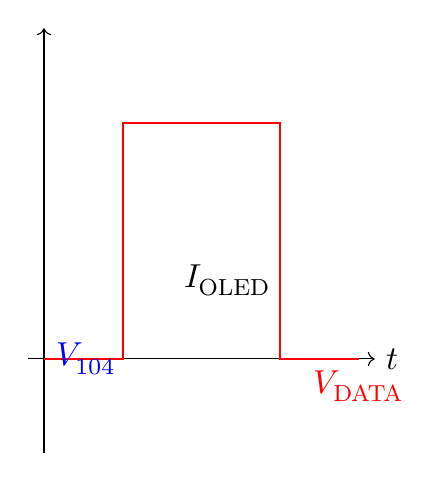
\begin{tikzpicture}[domain=0:4,samples=400]
    %\draw[very thin,color=gray] (-0.1,-1.1) grid (3.9,3.9);
    \draw[->] (-0.2,0) -- (4.2,0) node[right] {$t$};
    \draw[->] (0,-1.2) -- (0,4.2) ;
    \draw[thick, color=red] (0, 0) -- (1, 0) -- (1, 3) -- (3, 3) -- (3, 0) -- (4, 0)
    node[below] {$V_{\text{DATA}}$};
    \draw[thick, color=blue] plot[id=sin] function{x < 1 ? 0 :
      x < 3 ? 3 * (1 - exp(-1.8*(x-1))) : (3*(1-exp(-3.6))) * exp(-1.8*(x-3))} 
    node[right] {$V_{104}$};
    \draw[very thick,color=black] plot[id=exp] function{x < 1 ? 0 :
      x < 3 ? 2 * (1 - exp(-1.8*(x-1)))**2 : 2*(((1-exp(-3.6))) * exp(-1.8*(x-3)))**2} ;
    \node[black] at (2.33, 1) {$I_{\text{OLED}}$};
      \end{tikzpicture}
      \end{figure}
    \end{enumerate}

\end{enumerate}

\end{document}

